% Copyright 2018-2020 Melvin Eloy Irizarry-Gelpí
% \setcounter{chapter}{9}
\chapter{Centripetal Motion}
%
In this experiment you will study different aspects of centripetal motion.
%
\section{Preliminary}
%
So far, you have done experiments with objects moving in a single direction (like during free-fall motion) or back and forth (like going up and down on an inclined track, or bouncing off a spring loop). Besides such linear motion, you can have rotational motion where the direction of the motion changes continuously.

The simplest linear motion is with \textbf{constant velocity}: \textbf{uniform linear motion}. If the velocity is constant, then both its magnitude and direction are fixed in time.

The next simplest linear motion is with constant acceleration. Free-fall motion and motion on the incline are examples of this. Since acceleration is a vector quantity, constant acceleration implies constant magnitude and constant direction.

One of the simplest rotational motions is when an object moves along a \textbf{circular path} with a \textbf{velocity} vector that has a \textbf{fixed magnitude} $v$ but a direction that is constantly changing. It turns out that the \textbf{acceleration} vector of such an object also has \textbf{fixed magnitude} $a_{c}$ but constantly changing direction. The magnitude of this acceleration depends on the size of the circle and also on the magnitude of the velocity. Recall that a circle has a \textbf{radius}, which is defined as the distance from the center of the circle to any point on the circle. For an object in circular motion with constant velocity magnitude $v$ and moving in a circle with radius $r$, the magnitude of the acceleration vector is given by
\begin{equation}
    a_{c} = \frac{v^{2}}{r}
\end{equation}
This is known as the \textbf{centripetal acceleration}. If the object has mass $m$, then Newton's second law leads to the \textbf{centripetal force}:
\begin{equation}
    F_{c} = m a_{c} = \frac{m v^{2}}{r}
\end{equation}
You have sensors to measure \textbf{force} and \textbf{velocity}. The above relation suggest that for uniform circular motion you have
\begin{equation}
    F_{c} = \left(\frac{m}{r}\right) v^{2}
    \label{eq:10.Fc}
\end{equation}
That is, the amount of force acting on the object should be proportional to the square velocity. The constant of proportionality depends on the amount of \textbf{mass} and the size of the \textbf{radius} of the circle.

During uniform circular motion, the direction of the velocity vector is continuously changing. At any given moment in time, the velocity vector will be pointing in the direction that is tangential to the circle. The direction of the acceleration is also constantly changing, but it always points inwardly towards the center of the circle. Hence the name ``centripetal'' (i.e. center-pointing).
%
\section{Experiment}
%
The main goal of the experiment is to test the relation in (\ref{eq:10.Fc}) between the amount of force on the object and the square speed of the object. The slope depends on two quantities: mass and radius. To check this dependence, you performed two experiments:
\begin{enumerate}
    \item Keep radius fixed and change mass.
    \item Keep mass fixed and change radius.
\end{enumerate}
%
\section{Analysis}
%
Here are the steps to follow for the analysis.
%
\subsection{Visualize Force versus Velocity}
%
After each experiment you will collect velocity data from the photogate, and force data from the force sensor. It is good to make a chart with force in the vertical axis, and velocity in the horizontal axis. The chart \textbf{should not be linear}. In principle, a quadratic polynomial would be the best fit, but you do not have to do this.

You make this chart for at least one run, just to check the data.
%
\subsection{Visualize Force versus Square Velocity}
%
In a separate column on the spreadsheet, you can compute the square velocity values. Due to the manner in which the photogate measures velocity, the data does not consist of a velocity value for each force value. Suppose that column \texttt{B} has the force values, and column \texttt{C} has the velocity values. Suppose also that the force values begin in row \texttt{6}, such that the first force value is in cell \texttt{B6}. There is a chance that there will be no velocity value in cell \texttt{C6} (i.e. the cell is empty). The usual way to calculate the square velocity would be to write, in a separate column, something like this:
\begin{equation}
    \texttt{=C6\^{}2}
\end{equation}
and to then apply this operation to the rest of the velocity column. But since there are empty cells in the velocity column, the above operation will give zero for these empty cells. This way the square velocity column would consist of cells with square velocity values separated by cells with zero square velocity value. This is not right: for these zero square velocity values you have a corresponding non-zero force value!

You need to find the square velocity in a \textbf{conditional} way: if a cell in the velocity column is empty, then make the corresponding cell in the square velocity column also empty; otherwise calculate the square of the value. The following command accomplishes this:
\begin{equation}
    \texttt{=IF(C6="", "", C6\^{}2)}
\end{equation}
This way the square velocity column does not contain spurious zeroes.

Once the square velocity has been calculated correctly, you can make a chart with force in the vertical axis, and square velocity in the horizontal axis. The chart should now be linear. The best fit line will give you an equation of the form
\begin{equation}
    F = A v^{2} + B
\end{equation}
Here $A$ (the slope) should have units of force-divided-by-square-velocity, and $B$ (the intercept) should have units of force. If force is in N, and velocity in m/s, then $A$ should have units of
\begin{equation}
    \frac{\text{N}}{\text{m}^{2}\text{/s}^{2}} = \frac{\text{kg}}{\text{m}}
\end{equation}
and $B$ should have units of N. As discussed above, the slope of the chart should be close to the ratio of the amount of mass divided by the value of the radius. Since the intercept corresponds to the amount of force with zero velocity, the value of the intercept should be very small, corresponding to a force value that should be equivalent to noise, and thus effectively zero.
%
\subsection{Cut any Plateau Region}
%
For reasons that I am still trying to understand, the force sensor might yield a data set that exhibits a \textbf{plateau} (a flat region on a chart). This might be due to the force sensor saturating and not being able to properly record force data. For example, see Figure \ref{figure.10.run.1.before} where there is a plateau in the right hand side, for the larger force values. The plateau is having an undesirable effect because the linear fit is not appropriate.

It is safe to \textbf{cut the plateau} from the data set (as long as we assume the plateau is due to systematic error and not a real physical phenomenon). One way to consistently do this cut is to begin from the first row of data, and delete all the rows with a force value larger than 8 N. This is an informal \textbf{rule of thumb} and some times does not succeeds in cutting the plateau, meaning that forces less than 8 N should be cut (usually until 7.5 N). After doing such a cut, the chart should consist of a single linear segment, and the linear fit should be appropriate. For run 1, Figure \ref{figure.10.run.1} has the data after the cut. The linear fit is now much closer to the data.
%
\section{My Data}
%
Here is a breakdown of my runs:
\begin{itemize}
    \item Runs 1, 2, and 3: extra $m = 200$ g and $r = 10$ cm.
    \item Runs 4, 5, and 6: extra $m = 100$ g and $r = 10$ cm.
    \item Runs 7, 8, and 9: extra $m = 300$ g and $r = 10$ cm.
    \item Runs 10, 11, and 12: extra $m = 200$ g and $r = 8$ cm.
    \item Runs 13, 14, and 15: extra $m = 200$ g and $r = 12$ cm.
\end{itemize}
The corresponding expected values of the slope are found in Table \ref{table:10.m.r}.

The observed values for the slope and intercept are found in Table \ref{table:10.results}. As you can see from the second and third columns, the observed slopes are much larger than the expected values. The percent differences are consistently above 50\%, indeed closer to 60\%. Since this is true for all 15 runs, it appears that this outcome is due to a \textbf{systematic error}. Note that the slope values are consistent among repeated experiments.

This disagreement is embarrassing, but also serves as an opportunity to deal with systematic error. If you payed attention in class and repeated my steps, then very likely you found a similar disagreement in your data. Here is how I am quantifying the systematic error. Instead of the percent difference, I am going to calculate the ratio of the value of the slope that I observed from the data, to the expected value:
\begin{equation}
    \text{Ratio} = \frac{\text{Observed slope}}{\text{Expected slope}}
\end{equation}
This is done in Table \ref{table.10.ratio}. As you can see, the values in the last column are all close with an average value of 1.598. This means that, on average, the observed slope is about 1.598 times larger than the expected slope. That is, instead of getting the expected relation
\begin{equation}
    F = \left( \frac{m}{r} \right) v^{2}
\end{equation}
my data consistently implies that
\begin{equation}
    F = 1.598 \left( \frac{m}{r} \right) v^{2}
\end{equation}
There are five possible explanations for this result:
\begin{enumerate}
    \item The mass values are really 1.598 times larger than what I measured them to be. This is very unlikely.
    \item The radius values are really 1.598 times larger than what I measured them to be. This is not as unlikely, but plausible due to a bad configuration of the apparatus. Note that the radius value sets the scale for the velocity values.
    \item The force values are really 1.598 times smaller than what I measured them to be. This is puzzling, since you could expect the force measurements to disagree by an offset due to an improper zeroing, but not by a scale factor.
    \item A combination of the above effects.
    \item None of the above; something else.
\end{enumerate}
After searching online, I found a video from the makers of the equipment used in class, and it is clear that I did not followed the proper way of setting up the experiment. I still do not fully understand how any of the mistakes would lead to such a scale factor of 1.598. Last year I did not have this issue and the percent differences for the slope were very small (5\% to 15\%).

Even though there is great disagreement between the observed slope values and the expected slope values, the key facts about centripetal force were verified:
\begin{enumerate}
    \item The amount of force on an object moving in a circular path is proportional to the square velocity, as Figure \ref{figure.10.run.1} shows.
    \item When the mass of the object is increased, the slope also increases.
    \item When the mass of the object is decreased, the slope also decreases.
    \item When the radius of the circle is increased, the slope decreases.
    \item When the radius of the circle is decreased, the slope increases.
\end{enumerate}
I give myself a C- for this experiment. Sorry!
%
\section{Your Data}
%
You should have the following runs:
\begin{itemize}
    \item Runs 1, 2, and 3: extra $m = 200$ g and $r = 10$ cm.
    \item Runs 4, 5, and 6: extra $m = 100$ g and $r = 10$ cm.
    \item Runs 7, 8, and 9: extra $m = 300$ g and $r = 10$ cm.
    \item Runs 10, 11, and 12: extra $m = 200$ g and $r = 8$ cm.
    \item Runs 13, 14, and 15: extra $m = 200$ g and $r = 12$ cm.
\end{itemize}
The important thing about runs 7, 8 and 9 is that the extra mass value is larger than 200 g. Some students used 300 g, and others used 250 g. Both cases should yield the desirable outcome.
%
\newpage
\section{Your Laboratory Report}
%
Your lab report should include the following:
\begin{itemize}
    \item A table like Table \ref{table:10.m.r} with the mass values, the radii, and the expected slopes.
    \item A table like Table \ref{table:10.results} with your results.
    \item \textbf{One} chart with force in the vertical axis, and \textbf{velocity} in the horizontal axis. You are free to choose which run.
    \item \textbf{Five} charts with force in the vertical axis, and \textbf{square velocity} in the horizontal axis. One chart from runs 1, 2, or 3; one chart from runs 4, 5, or 6; one chart from runs 7, 8, or 9; one chart from runs 10, 11 or 12; and one chart from runs 13, 14, or 15. You are free to choose which five runs to include in the lab report. You should cut any plateau from the data, if present.
\end{itemize}
You should also answer the following questions:
\begin{itemize}
    \item Is the linear fit appropriate for the force versus velocity chart?
    \item Is the linear fit appropriate for the force versus square velocity chart?
    \item What happens to the observed slope when the mass is decreased?
    \item What happens to the observed slope when the mass is increased?
    \item What happens to the observed slope when the radius is decreased?
    \item What happens to the observed slope when the radius is increased?
\end{itemize}
%
\newpage
\section{Tables}
%
\begin{table}[ht]
    \centering
    \begin{tabular}{|l|r|r|r|r|r|}
        \hline
        Runs & Cart $m$ (kg) & Extra $m$ (kg) & Total $m$ (kg) & $r$ (m) & $m / r$ (kg/m) \\
        \hline
        1, 2, and 3 & 0.0521 & 0.2 & 0.2521 & 0.1 & 2.521 \\
        4, 5, and 6 & 0.0521 & 0.1 & 0.1521 & 0.1 & 1.521 \\
        7, 8, and 9 & 0.0521 & 0.3 & 0.3521 & 0.1 & 3.521 \\
        10, 11, and 12 & 0.0521 & 0.2 & 0.2521 & 0.08 & 3.151 \\
        13, 14, and 15 & 0.0521 & 0.2 & 0.2521 & 0.12 & 2.101 \\
        \hline
    \end{tabular}
    \caption{Mass values and radii used, along with expected slope values}
    \label{table:10.m.r}
\end{table}
%
\begin{table}[ht]
    \centering
    \begin{tabular}{|l|r|r|r|r|}
        \hline
        Run & Expected Slope (kg/m) & Observed Slope (kg/m) & Intercept (N) & P.D. (\%) \\
        \hline
        1 & 2.521 & 4.1407 & \textminus 0.0583 & 64.25 \\
        2 & 2.521 & 4.0983 & \textminus 0.0493 & 62.57 \\
        3 & 2.521 & 4.0410 & \textminus 0.0135 & 60.30 \\
        \hline
        4 & 1.521 & 2.4436 & \textminus 0.0267 & 60.66 \\
        5 & 1.521 & 2.4216 & \textminus 0.0057 & 59.21 \\
        6 & 1.521 & 2.4016 & \textminus 0.0037 & 57.89 \\
        \hline
        7 & 3.521 & 5.6048 & 0.0341 & 59.18 \\
        8 & 3.521 & 5.5167 & 0.1128 & 56.68 \\
        9 & 3.521 & 5.5928 & 0.1266 & 58.84 \\
        \hline
        10 & 3.151 & 5.4076 & \textminus 0.0385 & 71.60 \\
        11 & 3.151 & 5.1893 & 0.0595 & 64.68 \\
        12 & 3.151 & 5.1779 & 0.0544 & 64.31 \\
        \hline
        13 & 2.101 & 3.2542 & 0.1626 & 54.90 \\
        14 & 2.101 & 3.2343 & 0.1480 & 53.95 \\
        15 & 2.101 & 3.1035 & 0.3134 & 47.73 \\
        \hline
    \end{tabular}
    \caption{Results for slope and intercept}
    \label{table:10.results}
\end{table}
%
\begin{table}[ht]
    \centering
    \begin{tabular}{|l|r|r|r|}
        \hline
        Run & Expected Slope (kg/m) & Observed Slope (kg/m) & Ratio \\
        \hline
        1 & 2.521 & 4.141 & 1.643 \\
        2 & 2.521 & 4.098 & 1.626 \\
        3 & 2.521 & 4.041 & 1.603 \\
        \hline
        4 & 1.521 & 2.444 & 1.607 \\
        5 & 1.521 & 2.422 & 1.592 \\
        6 & 1.521 & 2.402 & 1.579 \\
        \hline
        7 & 3.521 & 5.605 & 1.592 \\
        8 & 3.521 & 5.517 & 1.567 \\
        9 & 3.521 & 5.593 & 1.588 \\
        \hline
        10 & 3.151 & 5.408 & 1.716 \\
        11 & 3.151 & 5.189 & 1.647 \\
        12 & 3.151 & 5.178 & 1.643 \\
        \hline
        13 & 2.101 & 3.254 & 1.549 \\
        14 & 2.101 & 3.234 & 1.540 \\
        15 & 2.101 & 3.104 & 1.477 \\
        \hline
    \end{tabular}
    \caption{Ratio of observed slope to expected slope}
    \label{table.10.ratio}
\end{table}
%
\newpage
\section{Figures}
%
\begin{figure}[ht]
    \centering
    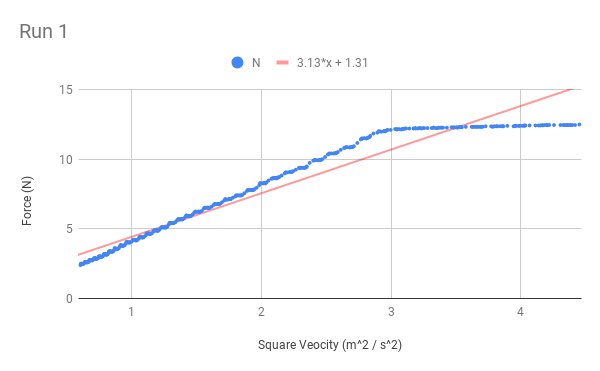
\includegraphics[scale=0.71]{image/10-centripetal/Run1BeforeCut.png}
    \caption{Run 1 before the cut; with plateau}
    \label{figure.10.run.1.before}
\end{figure}
%
\begin{figure}[ht]
    \centering
    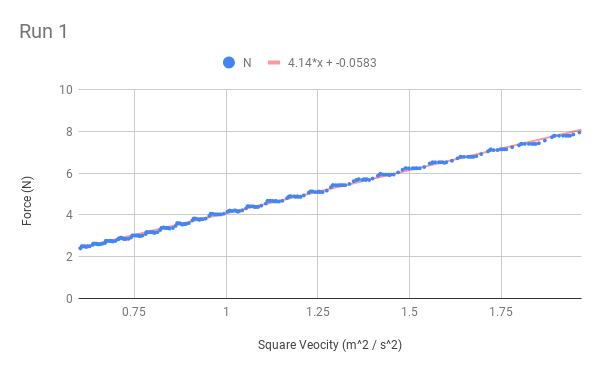
\includegraphics[scale=0.71]{image/10-centripetal/Run1.png}
    \caption{Run 1 after the cut; without plateau}
    \label{figure.10.run.1}
\end{figure}
%